\chapter{Исследовательская часть}
В текущем разделе будут представлены примеры работы разработанного программного обеспечения, постановка эксперимента и сравнительный анализ реализованных алгоритмов.

\section{Пример работы программного обеспечения}

На рисунке \ref{fig:prog_exmpl} представлен результат работы программы.

\begin{figure}[h!]
	
	\centering{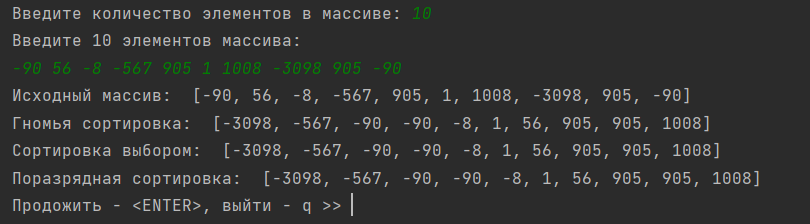
\includegraphics[scale=1]{inc/prog_exmpl.PNG}}
	
	\caption{Пример работы программы}
	
	\label{fig:prog_exmpl}
	
\end{figure}

\section{Технические характеристики}

Технические характеристики устройства, на котором выполнялось тестирование:

\begin{itemize}
	\item операционная система: Windows 10~\cite{windows10};
	\item оперативная память: 16 Гб;
	\item процессор: Intel® Core™ i5 10300H 2.5 ГГц.
\end{itemize}

Во время тестирования ноутбук был включен в сеть питания и нагружен только встроенными приложениями окружения и системой тестирования.

\section{Время выполнения реализаций алгоритмов}

Замеры процессорного времени реализованных алгоритмов сортировки (гномья сортировка, поразрядная сортировка, сортировка выбором) проводились с помощью функции process\_time() из библиотеки time языка Python. 

Функция process\_time() возвращает время в секундах (сумму системного и пользовательского процессорного времени).

Замеры времени для каждой длины массива (от 100 до 1000 элементов с шагом 200) проводились 100 раз для всех трех реализованных алгоритмов сортировки. В качестве результата бралось среднее время работы алгоритма на каждой длине массива.

Все реализации алгоритмов сортировки сравнивались на трех видах массивов: упорядоченный (лучший случай - все реализации алгоритмов сортировки выдают наименьшее время работы), упорядоченный в обратном порядке (худший случай - все реализации алгоритмов сортировки выдают наибольшее время работы), случайно сгенерированный массив (произвольный случай).

На рисунке \ref{fig:fig1} представлено сравнение процессорного времени работы реализаций алгоритмов сортировки на упорядоченных массивах (лучший случай).
На графике видно, что алгоритм сортировки выбором на данном виде массивов менее эффективен по времени, чем алгоритмы поразрядной сортировки и гномьей сортировки, которые практически одинаково эффективны по времени. Алгоритм сортировки выбором не зависимо от массива выдает сложность O(n$^2$).
\\
\\
\\
\\
\\
\\
\\
\\

\begin{figure}[h!]
	
	\centering{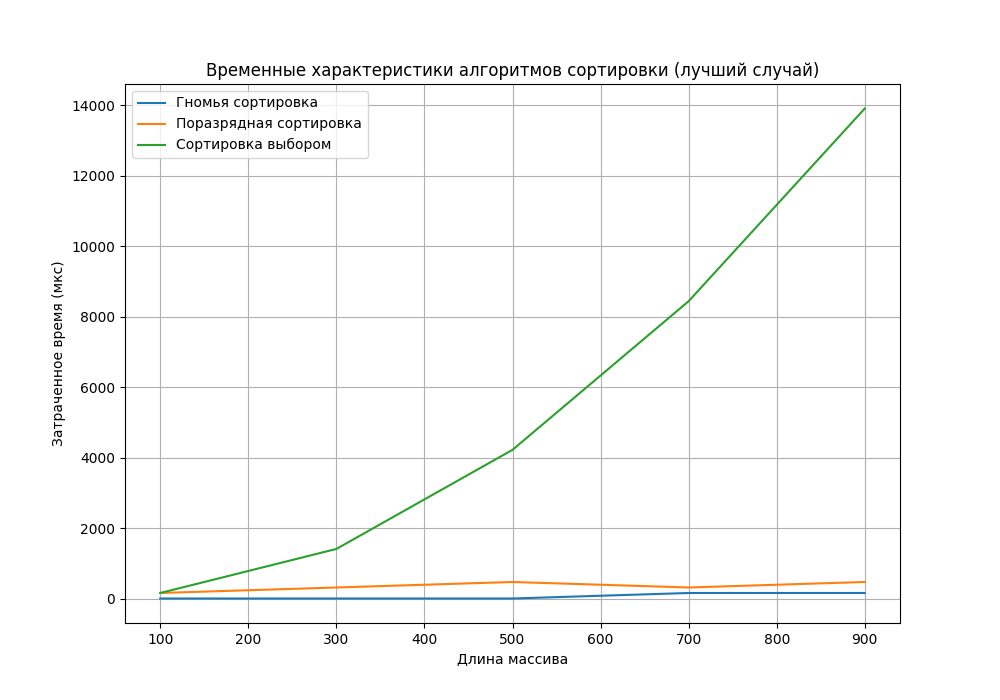
\includegraphics[scale=0.7]{inc/Figure_1.png}}
	
	\caption{Сравнение процессорного времени работы реализаций алгоритмов сортировки на упорядоченных массивах (лучший случай)}
	
	\label{fig:fig1}
	
\end{figure}

\FloatBarrier
На рисунке \ref{fig:fig2} представлено сравнение процессорного времени работы реализаций алгоритмов сортировки на упорядоченных в обратном порядке массивах (худший случай). На графике видно, что алгоритм гномьей сортировки на данном виде массивов является самым неэффективным по времени среди реализованных алгоритмов, на втором месте по эффективности - алгоритм сортировки выбором, на первом месте (самый эффективный по времени на данном виде массивов) - алгоритм поразрядной сортировки, причем его преимущество растет с увеличением длины массива.
\\
\\
\\
\\
\\
\\
\\

\begin{figure}[h!]
	
	\centering{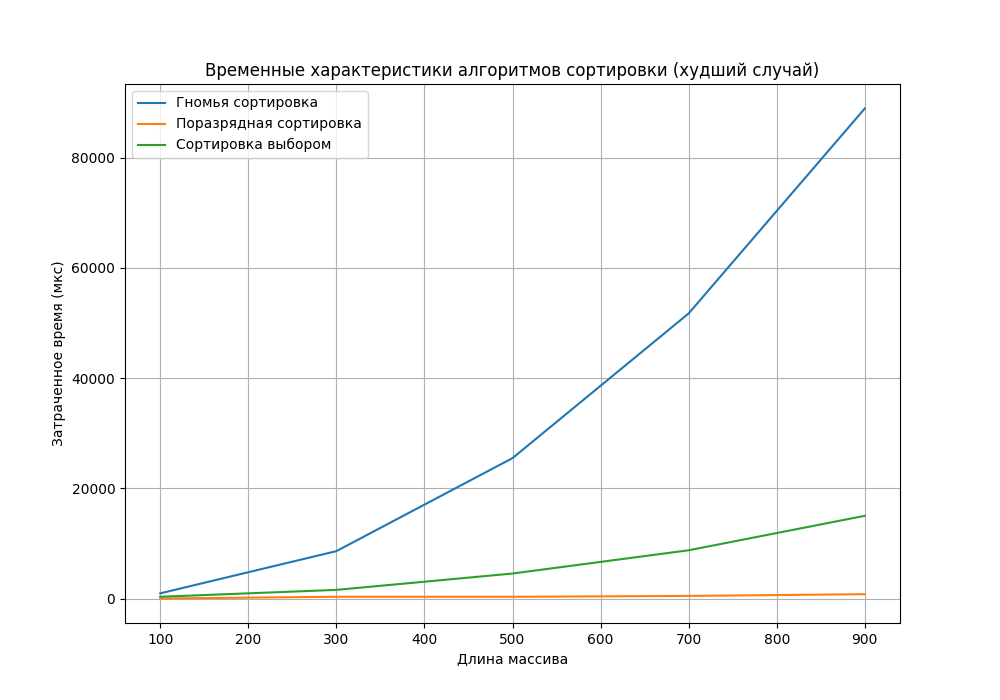
\includegraphics[scale=0.7]{inc/Figure_2.png}}
	
	\caption{Сравнение процессорного времени работы реализаций алгоритмов сортировки на упорядоченных в обратном порядке массивах (худший случай)}
	
	\label{fig:fig2}
	
\end{figure}

\FloatBarrier
На рисунке \ref{fig:fig3} представлено сравнение процессорного времени работы реализаций алгоритмов сортировки на случайно сгенерированных массивах (произвольный случай).
На графике видно, что алгоритм гномьей сортировки на данном виде массивов является самым неэффективным по времени среди реализованных алгоритмов,  на втором месте по эффективности - алгоритм поразрядной сортировки, на первом месте (самый эффективный по времени на данном виде массивов) - алгоритм сортировки выбором, причем его преимущество растет с увеличением длины массива.
\\
\\
\\
\\
\\
\\


\begin{figure}[h!]
	
	\centering{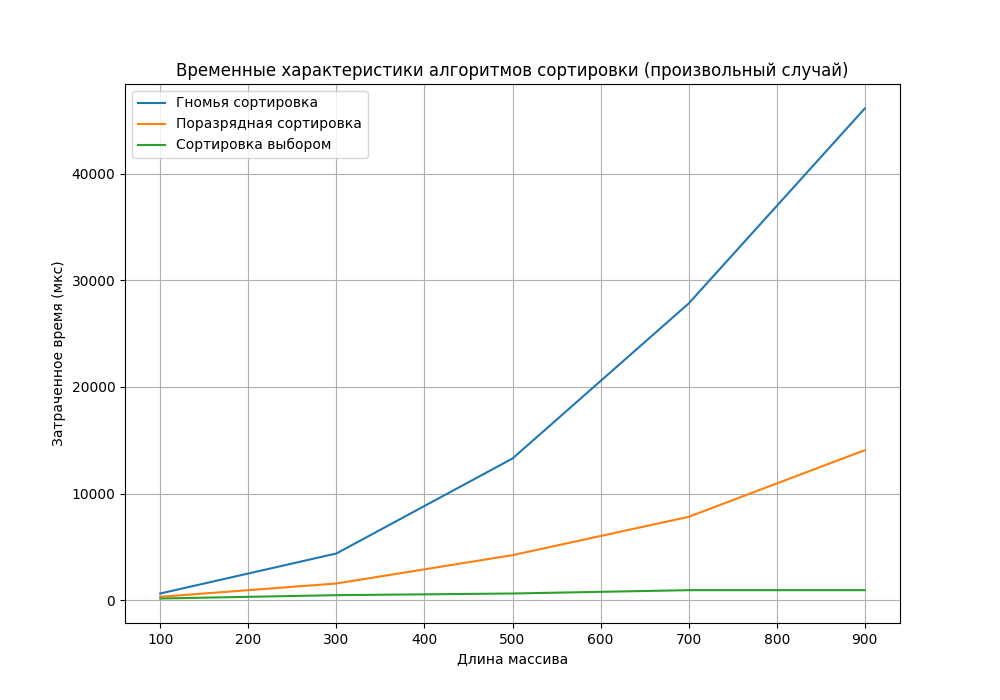
\includegraphics[scale=0.7]{inc/Figure_3.png}}
	
	\caption{Сравнение процессорного времени работы реализаций алгоритмов сортировки на случайно сгенерированных массивах (произвольный случай)}
	
	\label{fig:fig3}
	
\end{figure}

\FloatBarrier

\section*{Вывод}
Реализация алгоритма гномьей сортировки показывает худший результат среди реализованных алгоритмов сортировки по эффективности по времени в худшем и произвольном случаях и квадратично зависит от количества элементов в массиве, однако если массив уже был упорядочен, что бывает достаточно редко, реализация алгоритма гномьей сортировки показывает лучший результат наравне с поразрядной сортировкой.

Реализация алгоритма сортировки выбором является наиболее эффективной по времени в произвольном случае, однако в худшем случае проигрывает по эффективности по времени поразрядной сортировке, причем отставание растет с увеличением числа элементов в массиве. В лучшем случае сортировка выбором, наоборот, показывает худший результат среди реализованных алгоритмов.

Реализация алгоритма поразрядной сортировки является наиболее эффективной по времени в лучшем случае наравне с гномьей сортировкой и в худшем случае. В произвольном случае поразрядная сортировка уступает лишь сортировке выбором.

Таким образом, самой эффективной по времени по экспериментальным данным с учетом работы на всех видах массивов является поразрядная сортировка, но классическая реализация алгоритма поразрядной сортировки позволяет корректно сортировать только неотрицательные целые числа, для сортировки любых целых чисел или вещественных чисел потребуется модифицировать алгоритм.
